
\documentclass[12pt, letter]{article}
\usepackage[utf8]{inputenc}
\usepackage[spanish,es-tabla]{babel}
%\usepackage{times},puede ser arial 
\usepackage{csquotes}
\usepackage[left=2.54cm, right=2.54cm,top=2.54cm,bottom=2.54cm]{geometry}
\renewcommand{\baselinestretch}{1.5}
\usepackage[backend=biber,style=apa]{biblatex}
\bibliography{Referencias.bib}
\usepackage{graphicx}
\usepackage{subcaption}
\usepackage[hidelinks]{hyperref}

\title{\huge{Interrupciones}}
\author{Victor Manuel Arbeláez Ramírez \\ Facultad de ingeniería \\ Universidad de Antioquia}
\date{}

\begin{document}\raggedright

\maketitle

\section*{¿Qué es una interrupción en el contexto de los microprocesadores?}

\setlength{\parindent}{31pt}
Una interrupción consiste en un mecanismo que provoca la alteración del orden lógico de ejecución de instrucciones como respuesta a un evento externo, generado por el hardware de entrada/salida en forma asincrónica al programa que está siendo ejecutado y fuera de su control. 
\setlength{\parindent}{31pt}
Cuando se activa una interrupción, la próxima instrucción a ejecutarse no es la que se tenía prevista inicialmente en el del orden lógico, sino que se pasa a la primera instrucción de otro servicio o proceso causante de la interrupción. El programa de interrupción es semejante a una subrutina, ya que debe almacenar los datos de estado y registro para conservar el contenido del microprocesador antes de la interrupción.


\section*{¿Se puede hablar de la historia de las interrupciones?}

\setlength{\parindent}{31pt}
Se sabe que las interrupciones están presentes desde la aparición de los controladores basados en la arquitectura de von Neumann, ya que estaba la necesidad de interactuar con los periféricos externos mediante un software provisto de instrucciones al procesador. Inicialmente, la técnica que se empleo fue que el propio controlador se encargase de sondear el dispositivo cada cierta cantidad de tiempo "polling" para conocer en qué momento ejecutar algún proceso. Después, para ser más eficientes se optó propiamente por los conceptos de interrupciones, en donde se delega la responsabilidad al periférico para que avise de la necesidad de interrumpir un proceso para ejecutar otro.

\section*{¿Qué tipo de interrupciones existen?}

\setlength{\parindent}{31pt}
En general existen dos tipos de interrupciones, las externas e internas.Una interrupción externa es aquella que proviene de un dispositivo E/S (entrada / salida) y una interrupción interna es una compuerta de estado o un señalamiento dentro del microprocesador que pueden ser activados o desactivados mediante instrucciones de interrupción especiales. 

\setlength{\parindent}{31pt}
Cuando se desactiva una interrupción interna, el microprocesador no da servicio a interrupciones externas y cuando se atiende a una interrupción, lo primero que el microprocesador hace, es desactivar las interrupciones internas para evitar atender otras interrupciones.Aunque en algunos microprocesadores se presentan otro tipo de interrupciones, en donde cuentan con lineas de interrupción no enmascarables para hacer caso omiso al estado de interrupción interno y seguir aceptando interrupciones.

\begin{figure}[h!] %invoca una figura con el parámetro here
    \raggedright
        \begin{subfigure}[b]{0.45\linewidth}
            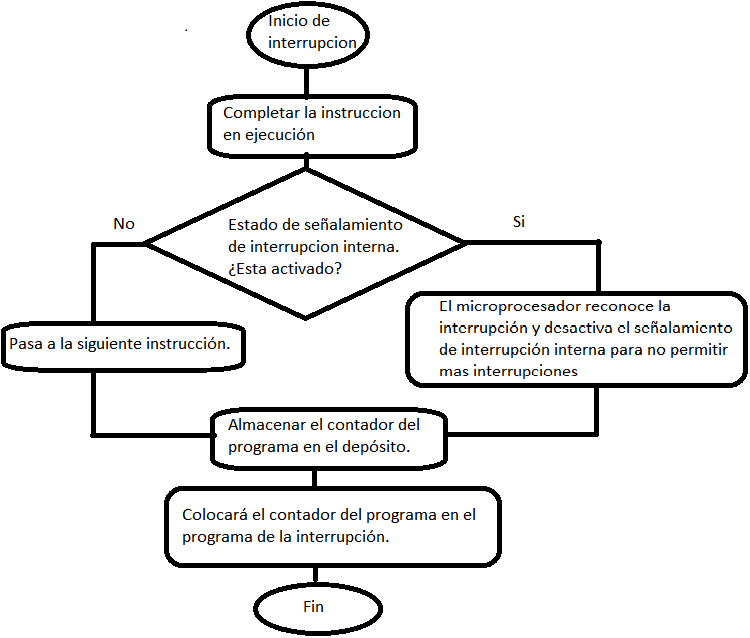
\includegraphics[width=0.8\linewidth]{Figuras/diagrama1.png}
            \caption{Comunicación típica del microprocesador}
            \label{fig:diagrama1}
        \end{subfigure}
    \raggedleft
        \begin{subfigure}[b]{0.45\linewidth}
            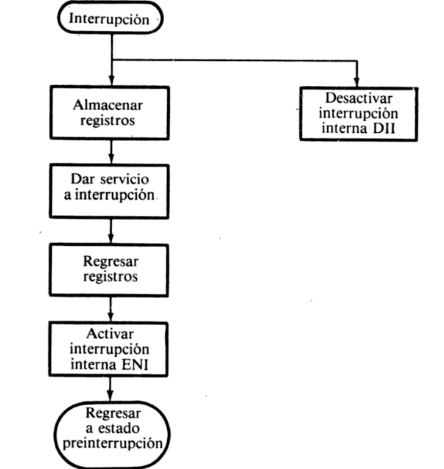
\includegraphics[width=0.8\linewidth]{Figuras/diagrama2.png}
            \caption{Secuencia del programa de interrupción}
            \label{fig:diagrama2}
        \end{subfigure}
    \caption{Diagramas de interrupciones}
    \label{fig:Diagramas}
\end{figure}

\setlength{\parindent}{31pt}
Normalmente en una comunicación con el microprocesador, responderá como se muestra  en la Figura ~\ref{fig:diagrama1}. Se presentan también interrupciones múltiples, en donde los dispositivos de micro procesamiento, generalmente están limitados en cuanto al número de conexiones y en ocasiones cuentan con algunas conexiones de señales dedicados para interrupciones. Cuando se requiere que una gran cantidad de dispositivos E/S, se interrelacionen con el sistema de micro procesamiento, las líneas de solicitud de estos dispositivos se someten a una operación “o” lógica, tal como se muestra en la Figura ~\ref{fig:diagrama2}.

\section*{¿Cómo se hace la implementación de interrupciones a nivel de hardware?}

\setlength{\parindent}{31pt}
Una interrupción por hardware es un mecanismo de comunicación entre el procesador y los dispositivos de E/S. Las interrupciones por hardware evitan que el sistema operativo tenga que muestrear periódicamente el estado de los dispositivos de E/S. El agente generador o solicitante de la interrupción activa la mencionada señal cuando necesita que se le atienda. Ante la solicitud de una interrupción, siempre y cuando esté habilitado ese tipo de interrupción, la unidad de control realiza un ciclo de aceptación para la interrupción. 

 \section*{ ¿Cómo se implementan las interrupciones por software?}

\setlength{\parindent}{31pt}
Es un mecanismo de comunicación entre un proceso (que se ejecuta en modo usuario) y el sistema operativo (que se ejecuta en modo supervisor). El proceso emplea las interrupciones por software para notificar al sistema operativo que requiere de su intervención. En procesadores x86, se ejecuta la instrucción int seguida de un número de 16 bits que indica el tipo de interrupción por software. Por ejemplo, las llamadas al sistema en x86 se implementan mediante interrupciones por software, por medio de la instrucción int 0x80 (sin embargo, hoy día las arquitecturas de los procesadores modernos vienen con instrucciones especializadas para la invocación de llamadas al sistema como syscall en x86, por tanto, esta técnica ha caído en desuso).  Para éstos procesos de interrupciones por software, se marca una mayor eficiencia cuando se utiliza el lenguaje ensamblador o lenguaje de máquina para comunicarse directamente con el microprocesador, pero también depende del hardware, ya que cada microprocesador tiene un numero determinado de pines para la función de interrupciones.

\printbibliography[title={Referencias}\nocite{*}]

\end{document}\raggedright
